\chapter{Introduction}
\label{sec:introduction}

Today, we use a number of computing devices interchangeably on a daily basis: a desktop workstation at the office,
a laptop computer on the move, a tablet in the living room and of course, always by our side, the smartphone.
In an increasingly cloudified and mobile world our expectation is to be able to do our work all the same,
regardless of the computing device we use, or where we are.

We start editing a text document in Google Docs on our desktop workstation at the office,
work on it a bit more on our laptop while travelling by train,
and proofread it later on the smartphone.
This device- and location-independent way of working has become the standard in recent years,
and users have started to expect it from their IT devices.

It's difficult to meet this expectation with the way electronic signatures are usually created today,
using certificates stored on on smartcards,
plugged into a laptop,
using a specialised card reader and accompanying software.
It's annoying and inconvenient having to carry around cables and adaptors, and a lot can go wrong:
a random operating system update breaking driver compatibility with the card reader, for example,
leaving us dead in the water.
If we want to make this easier on the user and to drive usage of electronic signatures and even make them mainstream,
we have to do better.

At the root of this inconvenience is the requirement that the user keep their private key physically with them,
stored in a manner making it difficult for anyone to steal it: on a smartcard.
Any IT professional knows full well this demand isn't made from users in order to annoy them but because it is
- more or less - the only practical \textit{and} secure way to have users store their private key.

So-called Remote Signing Services aim to eliminate the need for people to carry their private key with them,
and to locally create signatures,
in the hope for improved ease of use, and eventually, greater adoption of digitally signing documents.
However, allowing someone (the signing service, in this case) to be able to sign documents in place of the user introduces a number of serious security and confidentiality problems.


In this thesis, we analyse and address these problems,
and we implement the proposed solutions in a fully functional Remote Signing Service,
thereby showing that they work in the real world and not just on paper.

We will allow people to create electronic signatures,
no matter where they are, or what device they're using,
in a secure manner.
Building on our previous work of Project 2~\cite{projekt2}, we show how it is possible to securely integrate \gls{OIDC} authentication with remote digital signatures.
We expand upon this previous work and show how it is possible to have a remote signing service with the capability of signing on the users' behalf without the need for completely trusting that service.
Furthermore, we compare our solutions to those proposed by an industrial consortium led by Adobe Inc.,
and we show in which ways we believe our approach to be superior.

\subsection{Purpose of this document}\label{subsec:purpose-of-this-document}

In this document we will outline the objectives, scope and methodologies for our thesis as well as provide a project timeline.
The implementation will be documented separately.

\section{A cryptographic primer}\label{sec:a-cryptographic-primer}
In this section we well very briefly introduce the most important IT security and cryptography building blocks we use to make remote digital signing possible.
Readers with a basic knowledge of IT security topics such as hash functions, X.509, \gls{PKI} and \gls{DSA} can safely skip it.
The descriptions given are as brief as possible in order to introduce the topics, they're not meant to be complete nor excruciatingly precise.

\subsection{Hash Function}\label{subsec:hash-function}
A hash function in cryptography is an one-way function which is able to map data of arbitrary length to fixed-size values~\cite{hashing}.
One-way means that for a given hash value, it is infeasible to find the corresponding input data.
Ideally, the only way for someone to invert such a hash function is to do an exhaustive brute-force search.
This is called pre-image resistance.
Furthermore, a cryptographic hash function needs to fulfil the following properties:
\begin{enumerate}
    \item For a given input value, it must always produce the same hash value (it must be deterministic)
    \item It must be infeasible to find to different input values that produce the same hash value (this is called collision resistance)
    \item For a given input value, it must be infeasible to find another input value that produces the same hash value (second pre-image resistance)
    \item A minimal change in the input value must result in a completely different output value (avalanche effect)
\end{enumerate}

Hash functions fulfilling these properties are fundamental to our work (and to much of cryptography in general).
Without them we would be completely powerless.
An example for such a hash function is \gls{SHA-2}~\cite{sha2patent}.

\subsection{Asymmetric cryptography}\label{subsec:asymmetric-cryptography}
Asymmetric cryptography, sometimes called public-key cryptography, is a type of encryption which uses pairs of keys.
This is in contrast to symmetric encryption which uses only one key (for example, a passphrase encrypting a file).

With symmetric encryption the passphrase must me known both to encrypt and to decrypt the message,
but with public-key cryptography, the public key can be used to encrypt a message and the private key to decrypt it.

This might sound simple on the surface but opens up a world of possibilities.
Only the private key has to be kept secret, the public key can be freely published~\cite{stallings}.

The classical example for such an encryption system is the \gls{RSA} scheme~\cite{rsa}.

For a simplified example how public-key-based encrypted communication between two parties could work,~\footnote{
We're well aware of the major security problems in this example,
like the fact that both the key exchange and the message exchange happen unauthenticated and without integrity protection,
but we intentionally chose to keep the example as simple as possible in order to keep it easily comprehensible by a wide audience.
}
see figure~\ref{fig:simplepubkeycomm}.

\begin{figure}
    \centering
    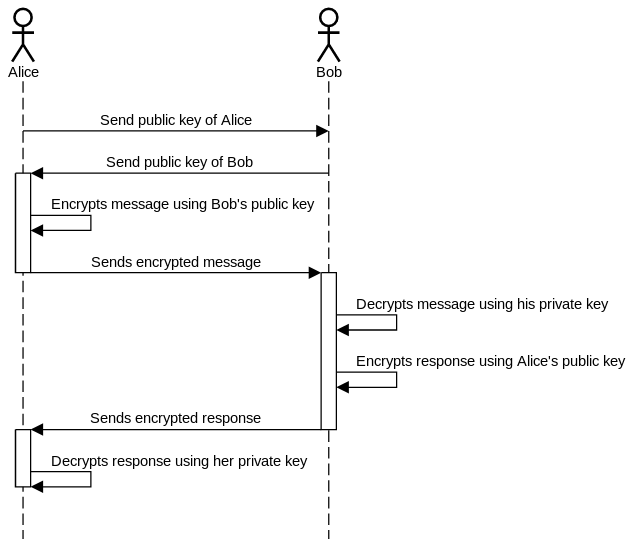
\includegraphics[width=0.75\textwidth]{images/simplistic_pubkey_communication.png}
    \caption{Simplified example of two Actors, Alice and Bob, exchanging encrypted messages using public-key cryptography}
    \label{fig:simplepubkeycomm}
\end{figure}


\subsection{Digital Signatures}\label{subsec:digital-signatures}
Having briefly explained Hash Functions in~\ref{subsec:hash-function} and Asymmetric Encryption in~\ref{subsec:asymmetric-cryptography} we can now move on to introducing digital signatures.
A digital signature is a way for verifying the integrity and authenticity of a message, that is,
to know who the message author is and to guarantee that it wasn't tampered with~\cite{digitalsignature}.

\paragraph{Digital Signatures are not Electronic Signatures}
Please note that the Digital Signatures we describe here are distinct from Electronic Signatures.
Electronic signatures provide the same legal standing as a hand-written signature on paper,
and as such are defined in laws such as ZertES~\cite{zertes}.
Digital signatures on the other hand merely refer to a mathematical scheme for providing message integrity and authenticity.
Digital signatures are used to implement electronic signatures, but they're not equivalent.


If we want to create a digital signature on a message, we perform the following steps:
\begin{enumerate}\label{enum:digitalsignaturecreation}
    \item We take our message and run it through a cryptographic hash function, thus obtaining the hash value.
    \item Then, we encrypt the hash value using our private key.
    \item We transmit the message and the encrypted hash value to the recipient.
\end{enumerate}

In order to verify the authenticity and integrity of the message, the recipient performs the following steps:
\begin{enumerate}
    \item They run the message through the same cryptographic hash function we did and obtain its hash value.
    \item They decrypt the encrypted hash value we sent them using our public key and compare it to the hash value they obtained themselves in step 1.
    \item If the values match, the recipient can be confident that a) the message wasn't tampered with and b) we authored it.
\end{enumerate}

In the message exchange shown in figure~\ref{fig:simplepubkeycomm},
there is a problem: anyone could encrypt messages for Bob and pretend to be Alice, since his public key is, well, public.

So by employing public-key cryptography, Bob is able to receive encrypted messages from Alice but they're of limited use to him,
since he has no way of knowing who actually sent them.
Fortunately, we can solve this problem by using digital signatures.

Before Alice encrypts her message to Bob using his public key,
she creates an digital signature by using a hash function and her private key as described above.
Then she encrypts both the message and the signature using Bobs public key and sends the two to him.

Bob then decrypts the message and verifies the digital signature as described above.

However, there is a serious problem still: an evil actor with the ability to intercept the communication
between Alice and Bob could not only read their messages,
but change them at will, effectively impersonating Bob as seen from Alice,
and Alice as seen from Bob.
For a solution to this problem please see section~\ref{subsec:digital-signatures}.

Figure~\ref{fig:pubkeymidm} expands upon figure~\ref{fig:simplepubkeycomm} to illustrate this attack.

\begin{figure}
    \centering
    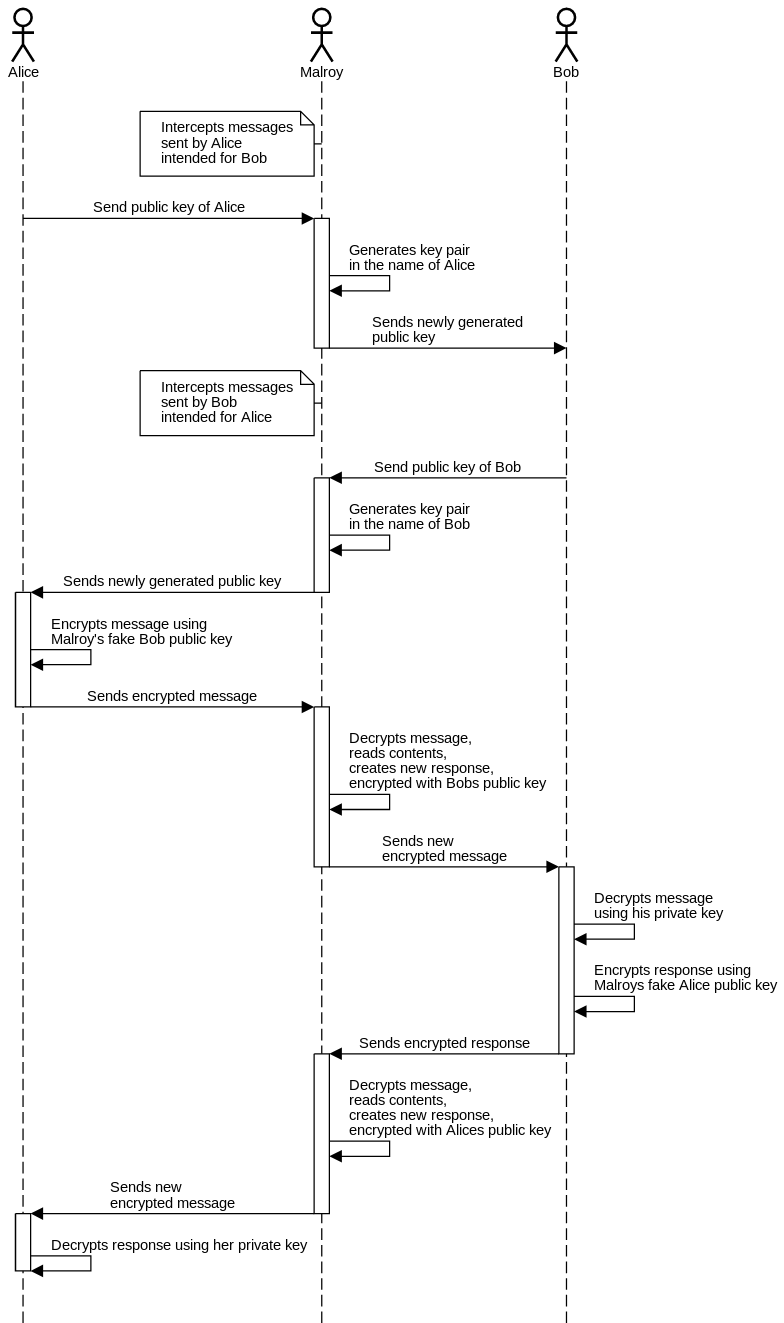
\includegraphics[width=0.85\textwidth]{images/pubkey_midm.png}
    \caption{Man in the middle attack on unauthenticated public-key encrypted communication}
    \label{fig:pubkeymidm}
\end{figure}


\subsection{Public-Key Infrastructure and Certificate Authorities}\label{subsec:public-key-infrastructure-and-certificate-authorities}
Public-key encrypted and authenticated communication as described in chapter~\ref{subsec:digital-signatures}
is vulnerable to man-in-the-middle attacks as illustrated in figure~\ref{fig:pubkeymidm}.
This attack works because Malroy is able to mislead Bob and Alice to use his keys instead of theirs
by intercepting their public keys in the initial key exchange.

This could be solved trivially if Alice and Bob exchanged their keys in a secure manner,
for example by meeting face-to-face,
thus ensuring Malroy can't sit in the middle.
However, this negates the main advantage of using public-key cryptography:
if they're forced to meet they could just as well exchange a symmetric key and use that for encrypting
their messages.

This one of the problems a \gls{PKI} solves.
On an abstract level, a \gls{PKI} is a mechanism that couples a public key with an identity~\cite{whatispki}.
What this means for the attack shown in figure~\ref{fig:pubkeymidm} is that it provides Alice and Bob
a way to make sure they're using each others' keys and not Malroys',
thus preventing the attack.
Because Alice and Bob now have a mechanism to verify which identity a public key refers to,
they can detect Malroys attack because the public keys maliciously issued by him will not correspond to Alice nor Bob.

A well-known and widely-used example for such a \gls{PKI} is X.509~\cite{x509}.
In practice such \gls{PKI}s are complex,
and because this section's already become longer than we like we'll forego explaining how X.509 works.

\subsection{Trusted Digital Timestamping}\label{subsec:timestamps}
Trusted digital timestamping is a scheme for proving the existence of a piece of information at a certain point in time.
There are several such schemes, such as X9.95 or ISO/IEC 18014.
In this section we will focus on \gls{PKI}-based timestamping as defined in RFC 3161~\cite{rfc3161}.

In RFC 3161, timestamps are issued by a trusted third party, the \acrfull{TSA}.

Trusted timestamps are created by using digital signatures (see~\ref{subsec:digital-signatures}) and hash functions (see~\ref{subsec:hash-function}).
In order to create a timestamp, the following steps are performed:
\begin{enumerate}
    \item We feed the information to be timestamped to a hash function and obtain its the hash value
    \item We send the hash value to the \gls{TSA}
    \item The \gls{TSA} concatenates the hash value with a timestamp
    \item The \gls{TSA} feeds the concatenation of our hash value with the timestamp to a hash function, in turn obtains the hash value of the concatenation
    \item The \gls{TSA} digitally signs the hash value from the previous step
    \item The \gls{TSA} sends the signed hash as well as the timestamp back to us
    \item We store the signed hash, the timestamp and the original information
\end{enumerate}
For an illustration of this process, see figure~\ref{fig:timestamping}

\begin{figure}
    \centering
    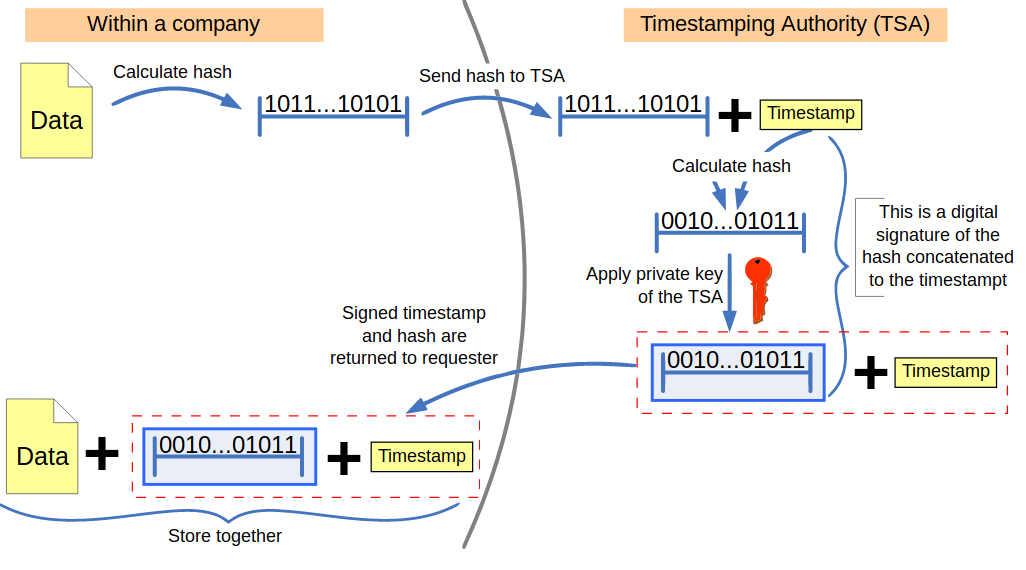
\includegraphics[width=0.85\textwidth]{images/timestamping.png}
    \caption{Process of obtaining a timestamp from a \acrfull{TSA}.
    Source: \url{https://en.wikipedia.org/wiki/File:Trusted_timestamping.svg}}
    \label{fig:timestamping}
\end{figure}

\subsection{Summary}
In a nutshell, the main ideas to take away from this chapter are:
\begin{itemize}
    \item Hash functions are one-way functions, mapping data of arbitrary length to fixed-length values
    \item Asymmetric cryptography allows for advertising the public portion of the key, and can be used to encrypt messages
    \item Digital signatures provide a means of verifying the integrity and authorship of a message
    \item Public Key Infrastructures provide a way to pair a public key with an identity
    \item Trusted Digital Timestamping is a means to proving the existence of a piece of information at a given point in time
\end{itemize}
